\documentclass[aspectratio=169, hideothersubsections]{beamer}
%\documentclass{beamer}
%\documentclass[aspectratio=1610]{beamer}
\usepackage{listings}
\usepackage{graphicx}
\usepackage{tikz}
\usetheme{Berkeley}
\usefonttheme{structuresmallcapsserif}
\usecolortheme{owl}
%\usepackage{xcolor}
%\usepackage{darkmode}
%\enabledarkmode
%\usecolortheme{albatross}
%\usecolortheme{spruce}
\usepackage{minted}
\usepackage{comment}
\usepackage{animate}  


\setbeamertemplate{page number in head/foot}[totalframenumber]
\setbeamertemplate{navigation symbols}{\footnotesize\usebeamertemplate{page number in head/foot}}
\setbeamercolor{title}{fg = OwlRed}
\setbeamercolor{author}{fg = OwlBlue}
%\setbeamercolor{frametitle}{fg=white}
%\setbeamercolor{background canvas}{bg=black}
%\setbeamercolor{normal text}{fg=white}

%--------------------------------------
%REPLACE IMAGE.JPG WITH LOGO OF ORGANISATION
\logo{\begin{tikzpicture}
\node[inner sep=0pt] at (0,0) {
\includegraphics[height=1cm]{SODS Logo.png}};
\end{tikzpicture}}
%--------------------------------------

\title{BSDS-208 : Image and Video Analytics}
\subtitle{Course Instructor - Mr. Aishwary Shukla}
\author[Gauri Sharan]{Gauri Sharan - BSc Data Science, Semester 4}
\date{June 11, 2024}

\begin{document}
\frame{\titlepage}

\begin{frame}{Table of contents}
    \tableofcontents[hideallsubsections]
\end{frame}

\section{Introduction}
\begin{frame}{Models of choice - Mediapipe's Models}{HandGestureClassifier and GestureRecognizer}
    \begin{itemize}
        \item MediaPipe is a cross-platform framework developed by Google for building multimodal machine learning pipelines. It supports a variety of domains such as vision, audio, and text.
        \item The framework is designed to facilitate the deployment of machine learning models on various devices including mobile phones, desktops, and the web, enabling real-time processing capabilities.
        \item MediaPipe offers a comprehensive set of pre-built solutions and tools to streamline the development process, making it easier for developers to implement advanced ML models in their applications.
    \end{itemize}
\end{frame}

\section{History}
\begin{frame}
    \frametitle{History}
    \begin{itemize}
        \item MediaPipe originated as an internal tool at Google, aimed at streamlining the development and deployment of machine learning models across various platforms.
        \item Recognizing its potential, Google released MediaPipe as an open-source project to enable the broader research and developer community to benefit from its capabilities.
        \item Since its release, MediaPipe has seen continuous development and integration of new features, expanding its applications in areas like hand tracking, face detection, and \alert{gesture recognition.}
    \end{itemize}
\end{frame}

\begin{frame}{History}
\begin{figure}
  \centering
  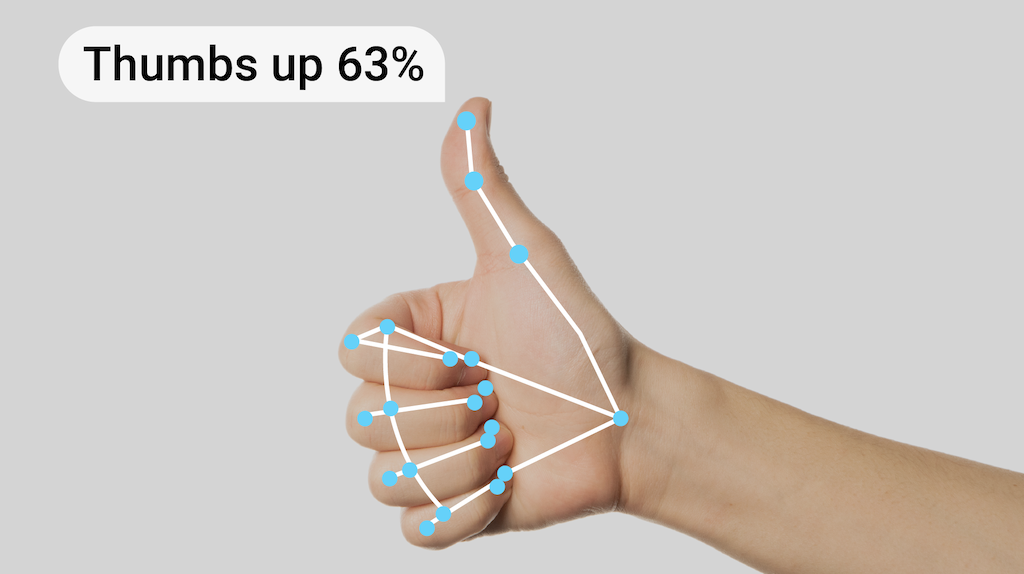
\includegraphics[width=0.6\textwidth]{key2.png}
  \label{fig:example}
  \caption{Hand gesture recognition using MediaPipe's Models}
\end{figure}
\end{frame}

\section{Research Analysis}
\begin{frame}
    \frametitle{Research Analysis}
    \begin{itemize}
        \item MediaPipe's gesture recognition models are grounded in cutting-edge research in computer vision and machine learning, utilizing convolutional neural networks (CNNs) and other advanced techniques.
        \item The models leverage extensive datasets to learn the nuances of hand movements and gestures, ensuring high accuracy and robustness.
        \item Research has shown that MediaPipe's models can achieve real-time performance with minimal latency, making them suitable for interactive applications.
    \end{itemize}
\end{frame}

\subsection{Insights}
\begin{frame}
    \frametitle{Insights}
    \begin{itemize}
        \item MediaPipe's models exhibit high accuracy in detecting and classifying hand gestures, which is crucial for applications requiring precise and reliable gesture recognition.
        \item The framework's cross-platform compatibility ensures that applications can be deployed on a wide range of devices without significant modifications.
        \item MediaPipe offers customization tools, allowing developers to fine-tune models according to specific datasets and use cases, enhancing the model's performance in targeted applications.
    \end{itemize}
\end{frame}

\subsection{Components Descriptions of Model}
\begin{frame}
    \frametitle{Components and Descriptions of Model}
    \begin{itemize}
        \item \textbf{HandGestureClassifier}: This model classifies gestures based on the detected landmarks of the hand. It maps the positions of key points on the hand to specific gestures using trained classifiers.
        \item \textbf{GestureRecognizer}: This model combines hand landmark detection with gesture classification. It first identifies key points on the hand and then uses these points to recognize specific gestures, providing a comprehensive solution for gesture recognition.
        \item Both models are built upon MediaPipe's robust hand tracking solution, which accurately detects and tracks hand landmarks in real-time.
    \end{itemize}
\end{frame}

\begin{frame}{Components and Descriptions of Model}
\begin{figure}
  \centering
  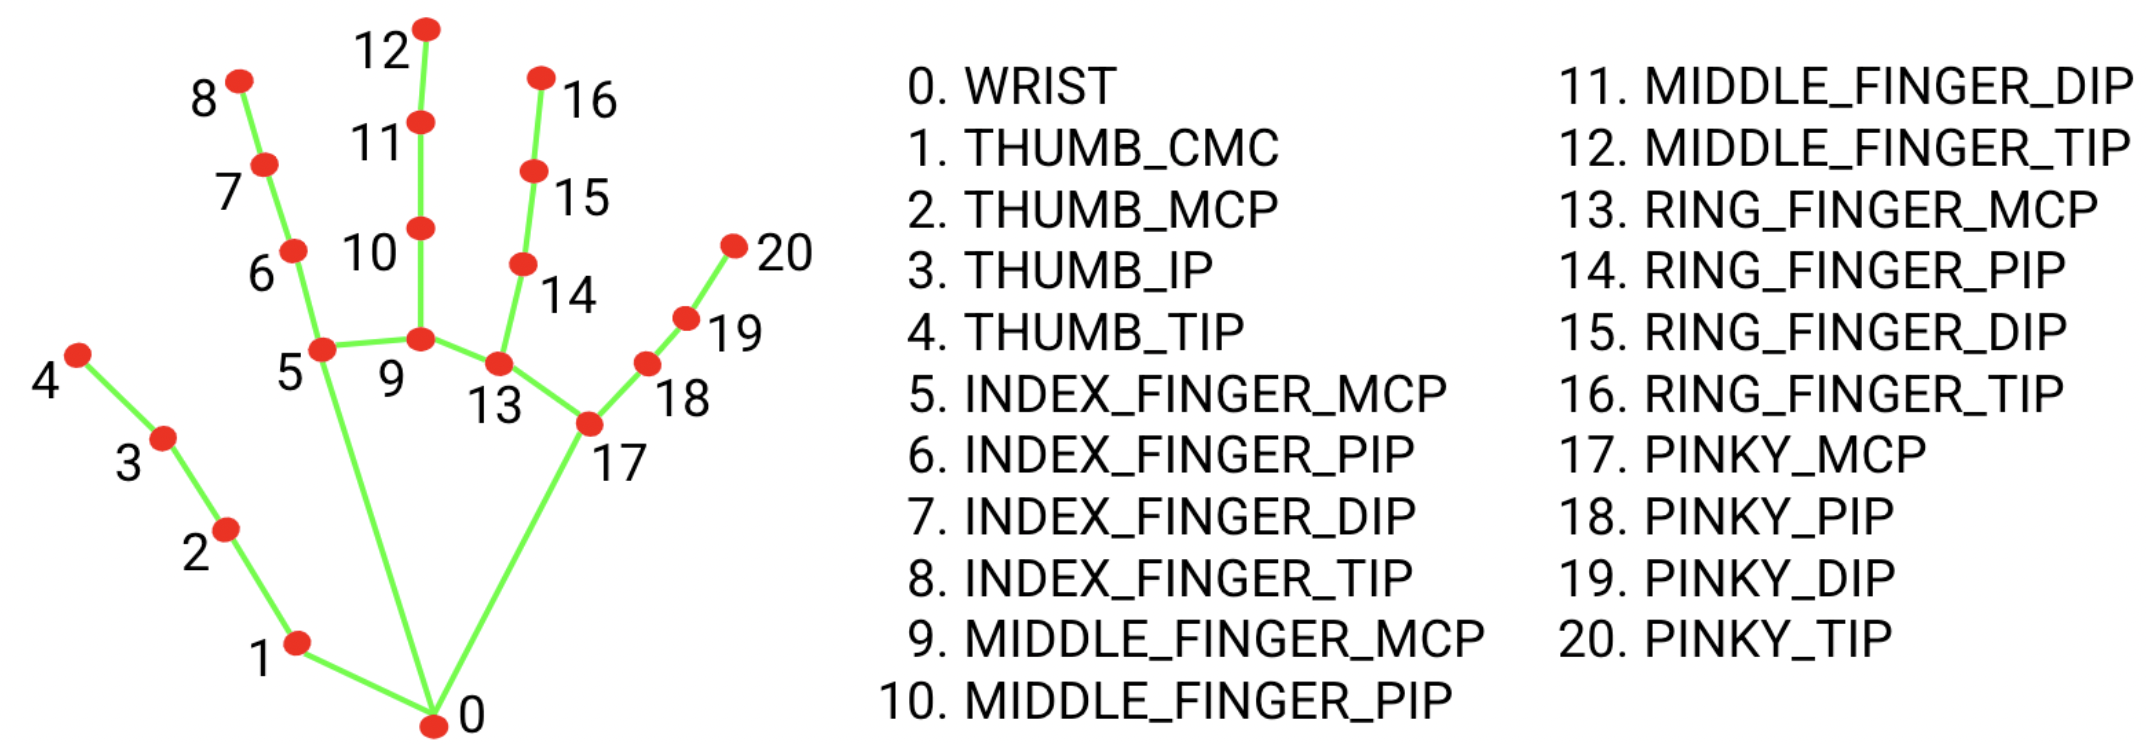
\includegraphics[width=0.7\textwidth]{key.png}
  \label{fig:example}
  \caption{HandGestureClassifier Model Landmarker Bundle}
\end{figure}
\end{frame}

\subsection{Architecture and Working of Model}
\begin{frame}
    \frametitle{Architecture and Working of Model}
    \begin{itemize}
        \item The architecture of MediaPipe's gesture recognition models consists of several stages, including hand detection, landmark localization, and gesture classification.
        \item Hand detection is performed using a CNN that identifies the presence of hands in the input image or video stream.
        \item Once hands are detected, a separate model locates the precise positions of key landmarks on the hands.
        \item These landmarks are then fed into a gesture classifier, which uses trained algorithms to recognize and classify the gestures.
        \item This multi-stage pipeline ensures high accuracy and real-time performance, making the models suitable for interactive applications.
    \end{itemize}
\end{frame}

\subsection{Training, Testing, Validation Hands-on}
\begin{frame}
    \frametitle{Training, Testing, Validation Hands-on}
    \begin{itemize}
        \item Training of the models involves using large datasets of hand images annotated with key landmarks and corresponding gestures. The models learn to identify patterns and features associated with different gestures.
        \item Testing is conducted on separate datasets that were not used during training to evaluate the model's performance and generalization capabilities.
        \item Validation involves cross-validation techniques where the data is split into multiple subsets. The model is trained on some subsets and validated on others to fine-tune parameters and improve performance.
        \item This rigorous process ensures that the models perform well in real-world scenarios and can handle diverse inputs effectively.
    \end{itemize}
\end{frame}

\section{Real Life Applications}
\begin{frame}
    \frametitle{Real Life Applications}
    \begin{itemize}
        \item \textbf{Sign Language Recognition}: MediaPipe's models can be used to develop applications that interpret sign language, facilitating communication for the hearing impaired.
        \item \textbf{Human-Computer Interaction}: Gesture recognition enables more intuitive and natural interactions with computers and smart devices.
        \item \textbf{Virtual Reality and Augmented Reality}: In VR and AR applications, gesture recognition allows users to interact with virtual environments in a more immersive and interactive way.
        \item \textbf{Interactive Gaming}: Gesture-based controls enhance gaming experiences, making them more engaging and interactive.
    \end{itemize}
\end{frame}

\section{Comparison}
\begin{frame}
    \frametitle{Comparison with Other Models}
    \begin{itemize}
        \item MediaPipe models offer superior real-time performance compared to traditional gesture recognition models, which may struggle with latency issues.
        \item The framework's cross-platform support provides an advantage over models designed for specific environments, such as desktop-only or mobile-only solutions.
        \item MediaPipe's customization options allow developers to adapt the models to their specific needs, providing more flexibility and efficiency compared to other less adaptable models.
    \end{itemize}
\end{frame}

\section{Customization}
\begin{frame}
    \frametitle{Customization}
    \begin{itemize}
        \item MediaPipe models can be customized using the MediaPipe Model Maker, which simplifies the process of training models with custom datasets.
        \item Developers can retrain models on their specific datasets to improve accuracy and performance for their particular use cases.
        \item Customization involves minimal code changes, making it accessible even to those with limited machine learning expertise.
        \item This flexibility allows developers to create highly specialized models tailored to their specific needs.
    \end{itemize}
\end{frame}

\section{Code Example}
\begin{frame}[fragile]{Python Code Example}
\rule{\textwidth}{1pt}
\scriptsize
\begin{minted}{python}
import mediapipe as mp
from mediapipe.tasks.python import vision

# Load the hand gesture recognizer
gesture_recognizer = vision.GestureRecognizer.create_from_model_path('path_to_model.tflite')

# Use the recognizer with an image
image = mp.Image.create_from_file('hand_image.jpg')
recognition_result = gesture_recognizer.recognize(image)

# Print recognized gestures
for gesture in recognition_result.gestures:
    print(f'Gesture: {gesture.name}, Confidence: {gesture.score}')
\end{minted}
\rule{\textwidth}{1pt}
\end{frame}

\section{Project}
\begin{frame}{Project}
  Project Link: \href{https://github.com/gaurisharan/gesture-recognition-mediapipe}{\bf github.com/gaurisharan/gesture-recognition-mediapipe} 
  Observed Output:
\begin{figure}
  \centering
  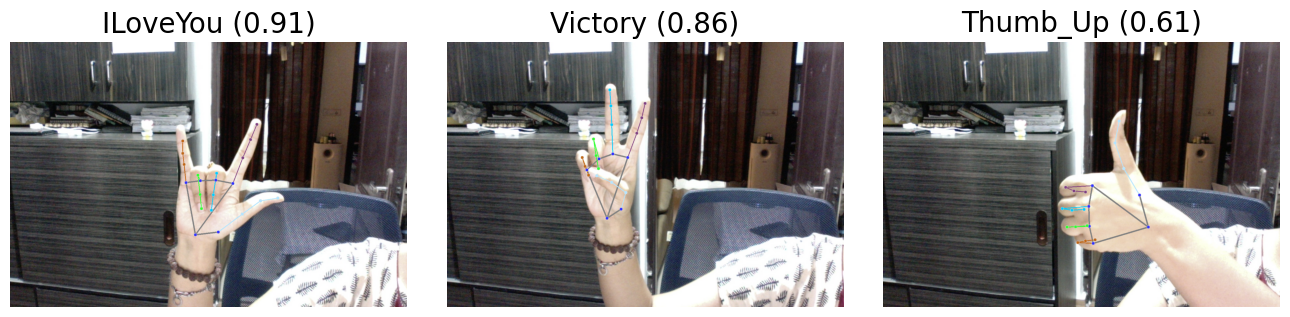
\includegraphics[width=\textwidth]{output.png}
  \label{fig:example}
  \caption{Gesture Recognition Model Output}
\end{figure}
\end{frame}

\section{References}
\begin{frame}{References}
  \begin{thebibliography}{10}
    \beamertemplatebookbibitems
    \bibitem{ref1}MediaPipe Framework. \textit{Official Website}. \url{https://ai.google.dev/edge/mediapipe/solutions/vision/gesture_recognizer}
    \beamertemplatebookbibitems
    \bibitem{ref2} MediaPipe Solutions. \textit{Official website}. \url{https://ai.google.dev/edge/mediapipe/solutions/customization/gesture_recognizer}
  \end{thebibliography}
\end{frame}

\section{Thank You}
\begin{frame}{Thank You}
Hope you liked this presentation. \newline \newline
\alert{Gauri Sharan} \newline
Student, School of Data Science \newline
AAFT Noida (Shobhit University) \newline
BSc Data Science 2022-25 \newline
Semester 4, 2024 \newline
\begin{itemize}
    \item LinkedIn: \href{https://www.linkedin.com/in/gauri-sharan}{\bf linkedin.com/in/gauri-sharan} 
    \item GitHub: \href{https://github.com/gaurisharan}{\bf github.com/gaurisharan}
    \item Mail: \href{mailto:gaurisharan123@gmail.com}{\bf gaurisharan123@gmail.com}
\end{itemize}
\end{frame}

\end{document}
